\section{Data Warehouse Reference-Architecture}
\label{sec:referenceArchitecture}
To order to have a common understanding about the topic of Data-Warehouse-Systems it is useful to quickly elaborate their fundamentals. Due to that the discussions and the considerations are easier to understand.\newline
Therefore the term ''DWS'' will be defined and its responsibilities will be delimited. Afterwards an architecture will be introduced which will be taken as reference during this paper.

\subsection{Defining the Data-Warehouse-System}
Before elaborating the reference architecture let's have a look upon the term 'Data Warehouse' itself and understand its process.\newline
This term was introduced around the end of the 1980s by William H. Inmon who is considered as father of this concept.
\begin{definition}
'A data warehouse is a subject-oriented, integrated, nonvolatile and time-variant collection of data in support of management's decisions.'\cite{buildingTheDWS}
\end{definition}
This results into a system which needs to be capable of retrieving, prepare and supply data for analysis.\newline
Now lets face the process needed to achieve that. The official term for that is 'Data Warehousing' which contains a process with six steps. [\cite{dwsRefArchitecture}, p. 9]
\begin{enumerate}
    \item Identify changes in relevant data form source systems
    \item Extract this relevant data from those systems
    \item Integrate, transform and clean up the extracted data
    \item Load the data into the Data Warehouse and persist it
    \item Deploy/Provide the data to analytical applications 
    \item Support to run those analysis
\end{enumerate}

\subsection{Introducing the Reference Architecture}
A system which used to be called Data Warehouse System should support and implement those steps in its software components. While developing such a DWS architectures, there leads no way around discussing the most commonly used reference explained by A. Bauer in his book 'Data Warehouse Systems'.\cite{dwsRefArchitecture}\newline
\begin{figure}[htb]
    \centering
    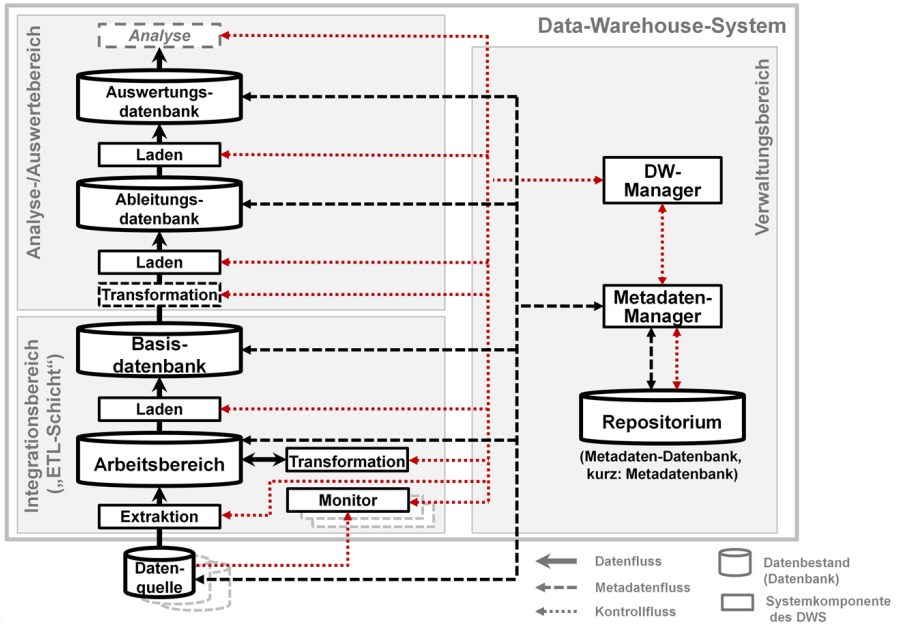
\includegraphics[scale=0.45]{pictures/DataWarehouseReferenceArchitecture.png}
    \caption{Reference architecture for Data Warehouse Systems by A. Bauer \cite[p.~42]{dwsRefArchitecture}}
    \label{fig:referenceArchitecture}
\end{figure} 

Now lets quickly go through the pictured software components and databases from figure \ref{fig:referenceArchitecture} starting at the bottom within the Extract-Transform-Load(ETL)-Layer. In order to retrieve data from several source systems with distinct technologies, a more complex extraction component is needed. This can be triggered by a monitor which scans for data changes in those data sources.\newline
After this step the whole data is loaded into a staging area in which a transformation happens. Two buzzwords in this context are data cleaning and cleansing. Therefore lets quickly elaborate the more complex data cleansing. 
'Data cleansing it the act of correcting or moving inaccurate, broken, or erroneous data from your data-set.'\cite{dataCleansing}
This step leads to the Core Data Warehouse which is basically a database containing all historic, cleaned, consolidated and analysis-neutral data samples. So concluded we can speak of an 'single source of truth'\cite{scriptRasch} which is a centralised and integrated database used as basis for further data handling and analysis.\newline
\\
The next part focuses upon the analytical-layer of the reference architecture. After loading the data from the core database into the derivation-database. This database is redundant to the core database but contains additional non-analysis-neutral derived data. Upon this database the data marts are build upon. Data Marts are just a slice of the whole amount of data. Additionally it is focused upon analysis and has therefore other data structures. In most use-cases multiple of those exist in order to have fast and detailed analysis of different areas inside the company.\newline
\\
On the right side of figure \ref{sec:referenceArchitecture} the management-layer is visualised. It contains components for managing the sequence- and data-flow and the metadata repository itself.\newline
\\
This should have described the fundamental ideas and concept of such a data warehouse system quite well without going into depths. The shown approach is closely related to Inmons hub and spoke architecture which will be introduced in the next section. 
